%&latex
\documentclass[12pt]{article}
\usepackage{amsthm,amsmath}
\usepackage{graphicx,psfrag,epsf}
\usepackage{enumerate}
\usepackage{natbib}
\usepackage{url} % not crucial - just used below for the URL
\usepackage{amsthm,amsmath}
\usepackage[utf8]{inputenc}

%\pdfminorversion=4
% NOTE: To produce blinded version, replace "0" with "1" below.
\newcommand{\blind}{1}

% DON'T change margins - should be 1 inch all around.
\addtolength{\oddsidemargin}{-.5in}%
\addtolength{\evensidemargin}{-.5in}%
\addtolength{\textwidth}{1in}%
\addtolength{\textheight}{1.3in}%
\addtolength{\topmargin}{-.8in}%


\begin{document}

%\bibliographystyle{natbib}
%\bibliographystyle{bmc-mathphys}
\bibliographystyle{agsm}

\def\spacingset#1{\renewcommand{\baselinestretch}%
{#1}\small\normalsize} \spacingset{1}


%%%%%%%%%%%%%%%%%%%%%%%%%%%%%%%%%%%%%%%%%%%%%%%%%%%%%%%%%%%%%%%%%%%%%%%%%%%%%%

\if0\blind
{
  \title{\bf Approachable case studies support learning and reproducibility in data science: An example from evolutionary biology}
  \author{Luna L. Sanchez Reyes\thanks{
    The authors gratefully acknowledge ``Sustaining the Open Tree of Life'',
    NSF ABI No. 1759838, and ABI No. 1759846. They are also also deeply grateful towards
    ``The Carpentries'' organization; without its invaluable volunteers and resources
    this project could not have been possible}\hspace{.2cm}\\
    School of Natural Sciences, University of California, Merced\\
    and \\
    Emily Jane McTavish \\
    School of Natural Sciences, University of California, Merced}
  \maketitle
} \fi

\if1\blind
{
  \bigskip
  \bigskip
  \bigskip
  \begin{center}
    {\LARGE\bf Approachable case studies support learning and reproducibility in data science: An example from evolutionary biology}
\end{center}
  \medskip
} \fi

\bigskip
\begin{abstract}
Research reproducibility is essential for scientific development. Yet, rates of reproducibility are low, especially in the natural sciences.
As increasingly more research relies on computers and software, efforts for improving reproducibility rates have focused on making research products digitally available, such as publishing analysis workflows as computer code, and raw and processed data in computer readable form.
However, research products that are digitally available are not necessarily friendly for learners and interested parties with little to no experience in the field.
This renders research products unapproachable, counteracts their availability, and hinders scientific reproducibility.
To improve both short and long term adoption of reproducible practices in research, research products need to be made approachable for learners, the researchers of the future.

Using a case study within evolutionary biology, we identify aspects of research workflows that make them unapproachable to the general audience:
use of highly specialized language;
unclear goals and high cognitive load; and
content-focused descriptions.
We propose a set of principles to improve the unapproachable aspects of research workflows, and illustrate their application using an online teaching resource.
We elaborate on the general application of these principles for documenting not only research products but also teaching materials, to provide present learners and future researchers with tools for successful scientific reproducibility.
%> ** add a sentence on implications for teaching reproducibility

\end{abstract}

\noindent%
{\it Keywords:}  open science, R programming language, phylogenetics, Open Tree of Life, pedagogy, phylogenetics, datelife
\vfill

\newpage
\spacingset{1.45} % DON'T change the spacing!
\section*{Introduction}
\label{sec:intro}

Research reproducibility --the extent to which consistent results are obtained when
a scientific experiment or research workflow is repeated \citep{repdef2021}-- is a key aspect of the advancement of science, as it constitutes a minimum standard that allows understanding research products, i.e., methods, data, analysis, results, etc. \citep{piwowar2013value}, to determine their reliability and generality, and eventually build up scientific knowledge and applications based on those products \citep{king1995replication, peng2011reproducible, powers2019open}.
In the natural sciences, rates of reproducibility are low \citep{ioannidis2005most, prinz2011believe}, which has elicited concerns about a crisis in the field \citep{baker2016reproducibility}.

In response, the scientific community has been developing new principles and standards to incentivize cultural changes that support a long term improvement of reproducibility rates in the natural sciences \citep{peng2015reproducibility, wilkinson2016fair, miyakawa2020no}.
A standard for reproducibility that has received much attention is availability, which we define as a property denoting that a research product can be reached (acquired, copied, analyzed, processed and/or reused) at no financial, legal or technical cost \citep{arnold2019turing}, and without geographic, demographic, social or temporal barriers for the population \citep{fecher2014open}.

In this paper, we argue that research products that are digitally available are often unapproachable in practice, because they are not friendly for learners and interested parties with different levels of experience in the field.
Research products that are unapproachable counteract availability, and hinder reproducibility short and long term.
To support long term adoption of reproducible practices in the natural sciences, research workflows need to be made approachable for learners, the researchers of the future \citep{roland2002think}.

To elaborate on our thesis, we designed a case study within the research field of phylogenetics, a discipline within evolutionary biology.
We use our case study to identify barriers that have made research workflows largely unapproachable to a general audience in the natural sciences.
Then, we propose some principles for researchers to address these barriers, and create research workflows that are reproducible by a larger audience.
% ** describe/introduce reproducibility curriculum here
The principles proposed here can be generalized and integrated into the undergraduate and graduate school STEM curriculum, either for courses specialized in reproducibility or within other subject areas, as a necessary component of successful and impactful science.

%% \bigskip
%% \bigskip
%%
%% \noindent\fbox{%
%%     \parbox{\textwidth}{%
%%     \textbf{Box 1. The role of approachable research workflows in teaching reproducibility.}
%%       % Availability is defined as the fact or possibility that something can be bought,
%%       % used, or reached by someone \citep{availability2022cambridge}.
%%       % Accessibility is defined as "the fact of being able to be reached or obtained easily"
%%       % \citep{accessibility2022cambridge}
%%       % Yet, in practice, availability does not imply accessibility.
%%       Availability and accessibility are conceptually accepted as synonyms for ``the fact
%%       of being able to be reached" \citep{available-accessible2022cambridge}.
%%       However, accessibility's definition goes further and describes it as the
%%       ``fact of being able to be reached \textbf{easily}" \citep{accessibility2022cambridge}.
%%       A secondary definition of accessibility elaborates more on this: ``the quality
%%       of being \textbf{easy to understand}''.
%%
%%       What we realize from these definitions is that, in practice, something might
%%       be available but not necessarily accessible,
%%       hindering the realization of availability.
%%       To illustrate the practical difference between availability and accessibility we
%%       will use an allegory that goes like this:
%%
%%       ** Change marshmallow story to cake
%%
%%       ** Explain different types of barriers to accessibility within the example, then within science
%%
%%       ** Explain why we focus on psychological/social/pedagogical barriers
%%
%%       ** Gauging accessibility of a resource is tricky because it depends on an
%%       individual experience of what is in effect \textbf{easy} for someone.
%%       \textbf{Easy} is a subjective quality that fully depends on individual perceptions
%%       resulting from individual contexts.
%%       As a society we are moving towards validating and welcoming all human experiences.
%%       To improve accessibility levels in the natural sciences, it
%%       is important to account for the factors that are creating different experiences
%%       of what is \textbf{easy}.
%%
%%       ** Now, explain different types of barriers to accessibility in science
%%       (Jessica: Maybe say that lack of accessibility can be due to a number of
%%       factors (physical, resources, economic), but one critical factor is the use
%%       of impenetrable expert language.)
%%     }%
%% }
%% \bigskip

\section*{A case study from phylogenetics}
\label{sec:case}

Phylogenetics is a key discipline within evolutionary biology \citep{dobzhansky1973nothing}.
It focuses on investigating the history of shared ancestry of living and extinct organisms using biological data, and represents this evolutionary history with a diagram known as a phylogeny or phylogenetic tree (because it grows through time and appears to have branches; Figure \ref{fig:tree}).
Phylogenies provide the basis to study and understand all biological processes in an evolutionary context \citep{dobzhansky1973nothing}.
Hence, it follows that improving reproducibility rates in phylogenetics has the potential to positively impact research across the natural sciences.

\begin{figure}
\begin{center}
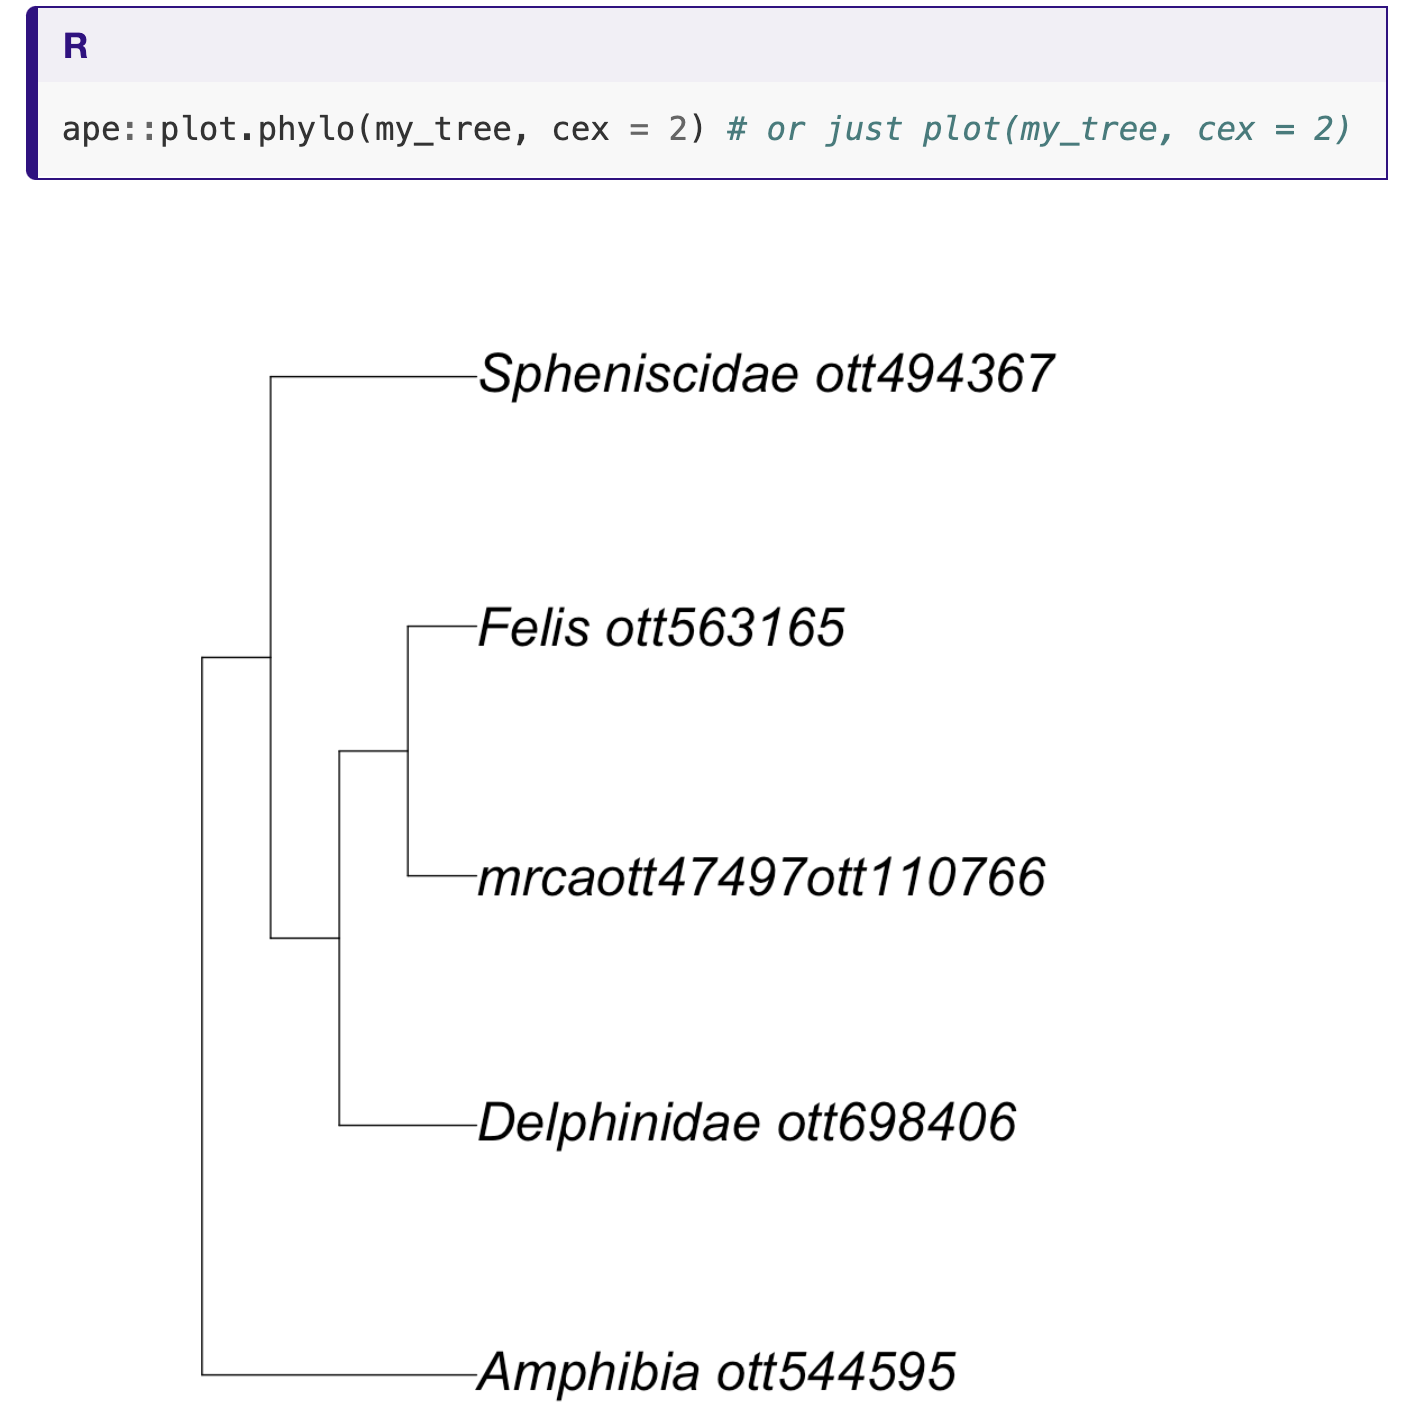
\includegraphics[width=3in]{fig_tree.png}
\end{center}
\caption{A phylogenetic tree from our tutorial. It was extracted using OpenTree of Life resources \citep{opentreeoflife2019synth} wrapped in the \texttt{rotl} R package \citep{michonneau2016rotl}. \label{fig:tree}}
\end{figure}

To explore barriers to approachable phylogenetics, we develop a case study that touches on three common problems within the field: standardizing organism names in phylogenies, obtaining current phylogenetic knowledge for a group of organisms, and summarizing this phylogenetic knowledge in a meaningful way.
To address these problems, we propose a research workflow that relies on resources from the Open Tree of Life (OpenTree), an open source project that provides digital availability of phylogenetic results from published, peer-reviewed research, which is considered as vetted and state-of-the-art knowledge in the field.
OpenTree phylogenies are stored in a public database, the Phylesystem \citep{mctavish2015phylesystem}, and are downloadable as various computer-readable file types, which is key for reusability and reproducible workflows \citep{wilson2017good}.
OpenTree also provides access to a single standard for organism names (taxonomic standard) that is applied to the stored phylogenies \citep{rees2017automated}, which are then used to summarize a single phylogenetic tree encompassing all life \citep{opentreeoflife2019synth}.

All of these resources
%% (the stored phylogenies, the taxonomic standard, the synthetic tree, and all
%% tools developed to process and summarize stored phylogenies),
are available for download and use from OpenTree free of cost to any user.
One way to access OpenTree resources is through its Graphical User Interface (GUI; aka, a website or application that allows users to access and use functionalities with mouse or keyboard clicks).
However, reducing as many manual steps as possible in research workflows is key for reproducibility, as manual data manipulation scales poorly and is prone to error \citep{bakken2019journey}.
OpenTree's resources are also programmatically available through its Application Programming Interface services (APIs; aka, computer code that implements computer functionalities, in this case OpenTree resources, that can be used by programmers
to build more functionalities), which provide scalability and reproducibility \citep{opentreeAPIv3}.
However, this comes at a high cost for the user, which requires considerably more computer programming experience and literacy to be able to successfully use APIs.
%% In recent years, OpenTree API services have been wrapped into software packages for R and Python
%% \citep{michonneau2016rotl, mctavish2021opentree}, open source, free of cost
%% programming languages that represent two of the most widely used programming languages
%% in the sciences \citep{baker2017scientific}. These packages should contribute to making
%% OpenTree resources more accessible to a wider user audience.
The \texttt{rotl} R package \citep{michonneau2016rotl} and the \texttt{opentree} Python module \citep{mctavish2021opentree} have been developed to wrap OpenTree's API services
and make them available through the R and Python programming languages.
R and Python are open source and free of cost, and represent two of the most widely used programming languages in the sciences today \citep{eglen2009quick, baker2017scientific}.
As such, \texttt{rotl} and \texttt{opentree} software packages should contribute to making OpenTree resources more accessible to a wider programming user audience.

However, while learners in the natural sciences have been engaging independently with R and Python programming languages, computer programming is not traditionally a core skill formally taught to biologists and naturalists \citep{sayres2018bioinformatics, wright2019the, williams2019barriers}.
As computers continue to play a larger role in most scientific disciplines \citep{piccolo2016tools}, higher baseline computational skills are required across all natural sciences not only to develop an original research workflow, but to be able to follow and reproduce research workflows from other researchers.

Thus, efforts to increase reproducibility rates long term in the natural sciences would benefit from addressing specific barriers for learners in the field, to support them in acquiring the skills needed to reproduce research workflows that rely heavily on computer code \citep{peng2011reproducible, sandve2013ten, powers2019open}.

In the next section, we describe (in no particular order) the barriers to approachable research workflows that we identified on our case study.
Then we develop a set of principles to address these barriers, and apply the latter to a set of teaching materials that are available at https://mctavishlab.github.io/R\_OpenTree\_tutorials/.


\section*{Identifying barriers to approachable research workflows}
\label{sec:identifying}

% Cite carpentries and Mosi

The main goal of our case study is to obtain a single phylogeny summarizing data from a set of published phylogenies for the canids (the family of dogs, coyotes, wolves, etc.), our organism of study.
All analysis for our case study can be completely accomplished using functions from the R package \texttt{rotl} or the Python module \texttt{opentree}.
If a researcher were to use the proposed analysis workflow in a publication, they would typically describe it in the methodology section as ``The canid summary phylogeny was obtained using functions from X package, details are available as supplementary files".
This is usual practice, mainly because journals do not have space to publish all code used for an analysis in the methods section. Yet, supplementary files and data have the misfortune to not be peer-reviewed as thoroughly (or at all) as the main manuscript \citep{pop2015use}.
They are also prone to the dreaded promise ``available upon request", which has very low rates of fulfillment \citep{krawczyk2012available}.
Without the primary data and code that was used to perform an analysis it is impossible to reproduce said analysis \citep{miyakawa2020no}. When the code is available, other issues can complicate reproduction of the analysis, to the point of completely obstructing reproducibility.
For example, some questions that are often unaddressed in research workflows are:
\textit{what software do I need to open the code files?}
\textit{Can I run the code with the same software I used to open the files, or do I need a different one?}
\textit{Do I need additional software that the analysis depends on?}
\textit{What does the code even mean?}

These questions can usually be answered by referring to the software documentation, which are usually publicly available and can be accessed by any potential user.
As opposed to code, software documentation is written in natural language (i.e., any known human language, e.g., English, Spanish, Chinese), and is considered a key element for successful adoption of software by target users \citep{karimzadeh2018top}. This might explain why documentation for software addressed to academic users is also usually written using highly specialized computational language or jargon (i.e., computationally specific concepts, words, and phrases) as well as formal scientific and academic language.
We identify this as \textit{barrier 1} to approachable research workflows.-- \textit{Specialized language is intimidating}.
While scientific jargon might have an important role for formal acceptance of software by the scientific and academic community, it can be perceived as cold and/or intimidating language, that often slows down or even obstructs examination, application, and adoption of code by a wider audience \citep{ball2017its}.
In contrast, introducing information without the use of jargon, supports learner's conceptual understanding of new ideas and concepts \citep{mcdonnell2016concepts, pan2019online}.
% jargon creates a hostile environment that does not foster learning \citep{CITATION}.

Another element of good software documentation is that it has to be thorough \citep{karimzadeh2018top}.
Meaning that it should describe general usage of individual functions, as well as arguments and variables that said function can take \citep{karimzadeh2018top}.
Individual documentation for each function is usually presented in alphabetic order, and does not have a specific analysis goal.
Moreover, most software has numerous functions, so documentation is usually very lengthy and it is hard to navigate.
This can have the effect of increasing the amount of information that needs to be simultaneously processed by the users, which can lead to overload of the finite amount of working memory any one possesses, known as cognitive load \citep{sweller1988cognitive}.
In this context, identifying connections across functions that are meant to work on the same analysis workflow can become a very difficult task.
We recognize this as \textit{barrier 2.-- Lack of specific goals leading to high cognitive load}.
High cognitive load is know to have a negative effect in learning software \citep{chandler1996cognitive, van2005research, lambert2009student}.

A third important aspect of software documentation are examples that demonstrate usage of individual functions \citep{karimzadeh2018top}.
Examples presented in software documentation are usually worked to perfection, as they are intended to showcase the ideal or minimal case in which a function works well.
Perfectly worked examples ignore the user experience by maintaining focus on the software content, and fail to provide users with expert and clear advice on how to troubleshoot if needed.
We identify this as \textit{barrier 3.-- Content-focused examples}.
Error management training is an approach that focuses on framing mistakes as beneficial to learning complex tasks, to give learners the opportunity to
actively explore a task with a positive mindset \citep{frese1995error}.
Providing examples that showcase potential errors supports user's performance \citep{steele2014error}, and can greatly improve learner's ability to troubleshoot outside the classroom \citep{shannon2015live, nederbragt2020ten}.

%% Last but not least, software documentation is usually explained verbally in a document, very
%% rarely is it approached using diagrams or other allegories.
%% We recognize this as \textit{barrier 4.-- Little to no diversity of representation of information}.

In sum, best practices for good software documentation are not enough to promote reproducibility of published research workflows that rely heavily on code.
In the following section we describe some principles that can help to reduce or remove the identified barriers, to create research workflows that are more approachable and hence more reproducible by a larger audience.

\section*{Principles for approachable research workflows}
\label{sec:addressing}

\subsubsection*{Principle 1. Use friendly, relatable and respectful language}

% avoid specialized, intimidating and cold language

Avoiding formal language, and incorporating elements of pop culture, such as picture character icons known as ``emojis``, make the language more familiar to a broader target audience (Figure \ref{fig:error}). We made an effort to specifically complement the primary documentation by identifying computational concepts that were assumed or were not explained in depth.
We vetted the tutorials through feedback from workshop participants as well as individual users to identify such specialized concepts.

\begin{figure}
\begin{center}
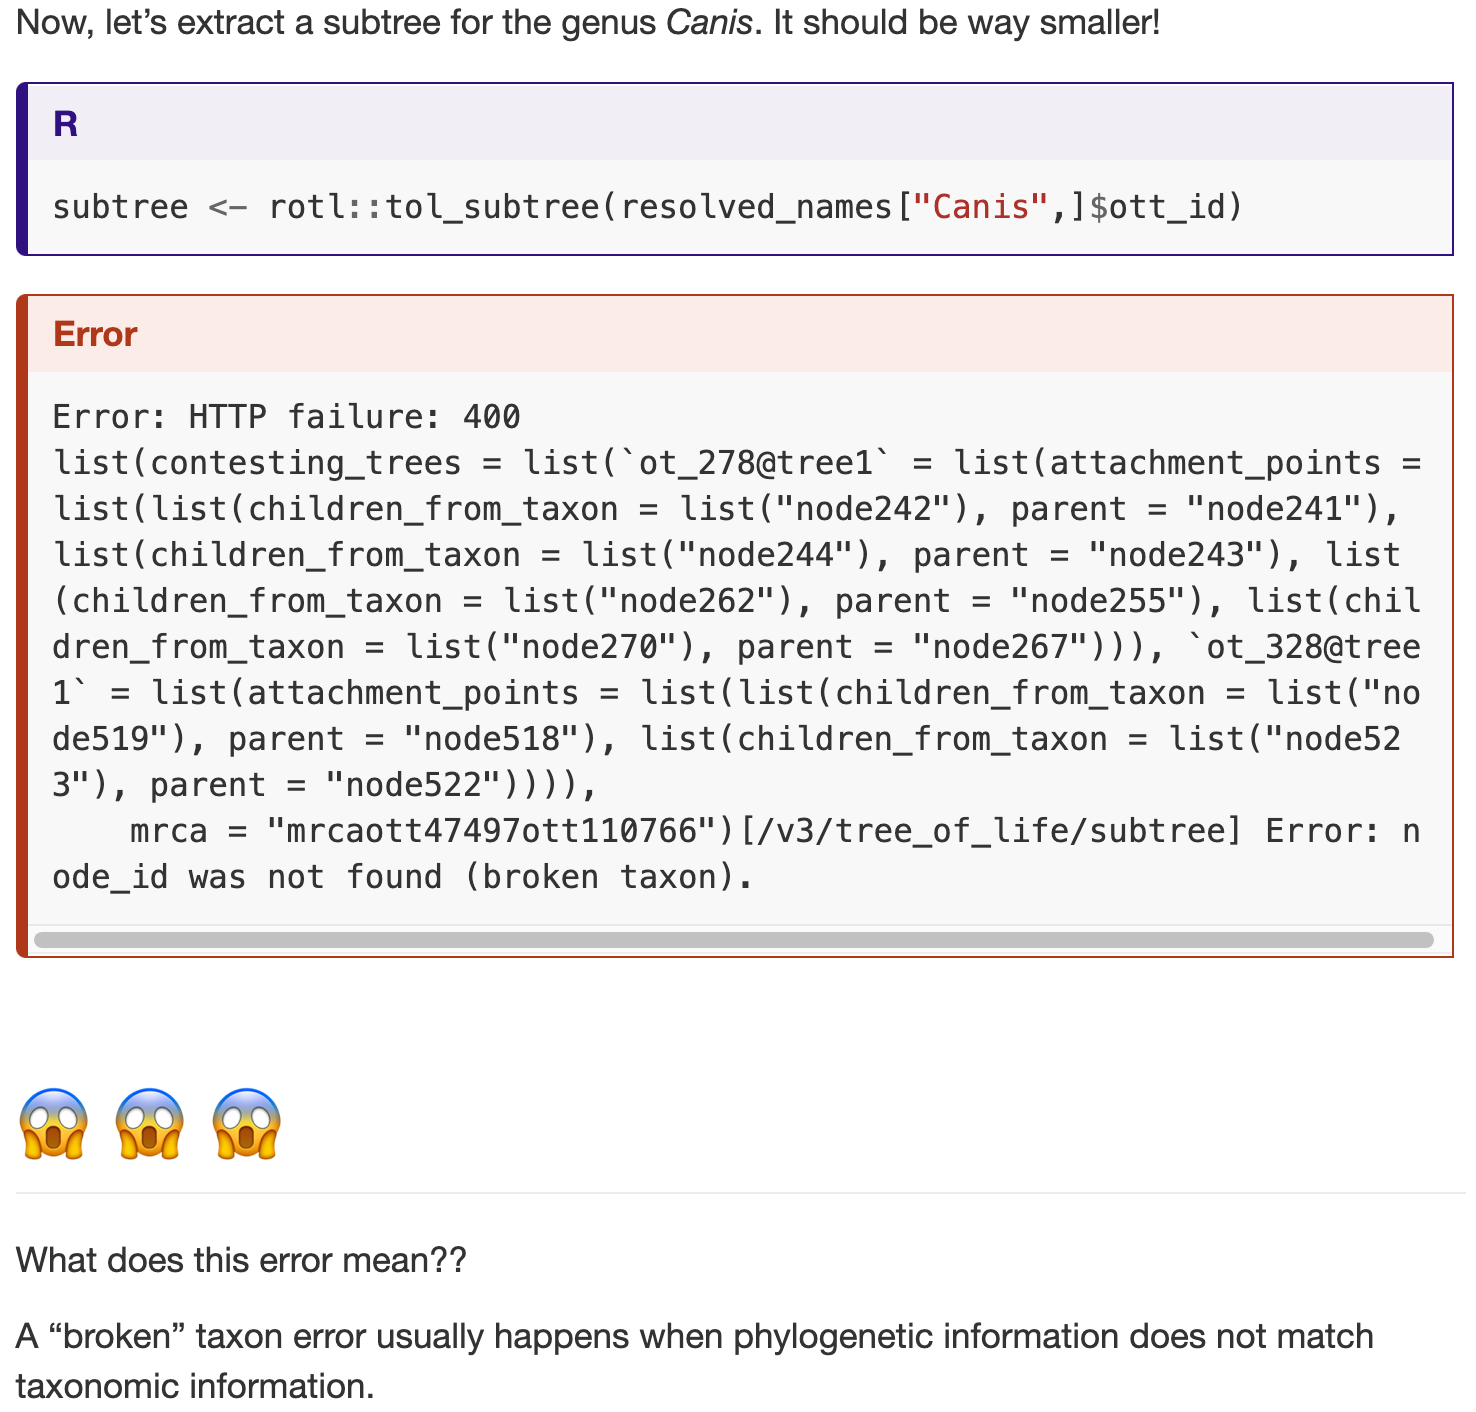
\includegraphics[width=3in]{fig_error.png}
\end{center}
\caption{Snapshot of a section of the tutorial website, where we demonstrate a common error. \label{fig:error}}
\end{figure}

\subsubsection*{Principle 2. Reduce cognitive load by providing specific and clear goals with literate programming}

Cognitive load can be greatly reduced for learners by applying an active learning strategy such as linking usage to a ``real world'' or ``human'' application \citep{felder2009active}.
Programming computer languages are by themselves quite abstract and represent a learning subject with a potentially high cognitive load for most learners.
Pedagogical research shows that active learning practices are one of the most effective ways to take on abstract subjects \citep{freeman2014active}.
A story-like narrative that links code usage in an integrative example, invites learners to try the code, which can lead them to remember what they are doing and why they are doing it.
This ``literate programming'' paradigm \citep{knuth1984literate, fritzson2002mathmodelica} makes code more approachable, as it integrates narratives with computer code in the same document, supporting learners in actively following the code usage, supporting memory and understanding \citep{piccolo2016tools}.

We propose that documents developed with ``literate programming'' can be made more accessible by choosing narratives that are relatable to a more general audience.
An easy way to do this in biology is choosing a charismatic taxon as a model organism.
For a research group, this can be the biological group they are studying. For the general audience, a highly charismatic group --such as dinosaurs, should work well.
For example, when we presented our tutorial to the Amphibia Web Organization \citep{van2002amphibiaweb} in January 2020, we tailored all examples to frogs and their allies.
% \citep{cite-aw-workshop}

We examined available software documentation for the package \texttt{rotl}, and designed a narrative that requires the usage of as many functions as possible.
We demonstrate code applications that are commonly requested by OpenTree users, but that are not demonstrated in the documentation of the package.
By framing the function workflow using highly requested uses, the documentation acquires a narrative arc that is easier to follow and remember by users.
This can also facilitate translating the code application to other use cases of interest for learners in biology.

%% Maybe Figure!! In the tutorial showcased here, we used the commonly requested
%% use case of obtaining
%% a phylogenetic tree for all lineages within a specific taxonomic rank.

\subsubsection*{Principle 3. Provide examples that are user-focused by demonstrating errors and warnings}

% approachable practice: user focused examples (instead of content focus)
% demonstrate errors and warnings thoroughly

An activity that has become increasingly widespread in programming-language education is live programming.
During live programming, an instructor writes code and executes it in a way that is visible to learners through a screen \citep{guzdial2013lure, selvaraj2021live}.
One benefit of this practice is that typos and mistakes occur, normalizing them for learners.
Watching an instructor handling errors, demonstrates learners on how to solve them when they are outside the classroom \citep{shannon2015live, nederbragt2020ten}.
When co-author McTavish was a postdoc, teaching an introductory programming workshop as a volunteer with the Carpentries (a non-profit group that teaches foundational coding and data science skills to researchers worldwide) \citep{wilson2006swc, SWCwebsite},
a senior faculty member taking the workshop complained that the typos were slowing things down and interfering with the pedagogy.
McTavish replied "the typos ARE the pedagogy".
This has become a slogan of sorts at the Carpentries, capturing the idea that embracing and discussing mistakes is essential to teaching programming \citep{wilson2019teaching}.
Yet, working through mistakes is rarely done on written pedagogical materials.
Software documentation focuses on demonstrating usage function with examples that work seamlessly, without errors.
We argue that the opposite is needed to support adoption of reproducible workflows and support long term independence in learner's and user's performance \citep{gaspar2007restoring, steele2014error}.

In our tutorials, we apply this principle by demonstrating examples that do not work as expected, and exemplifying ways to address issues (Figure \ref{fig:error}).
For example, we identified inputs that would give a wide range of warnings and errors.
We then focus on providing explanations for these errors and warning messages.
We believe this supports users and learners to be less intimidated by the messages, and to practice taking useful information out of them.
% This is probably part of the computer science curriculum, but it is not at all
% part of the natural sciences curriculum.

We also demonstrate ways to evaluate inputs to determine if they will trigger an error or warning, and design and demonstrate alternative analysis routes on what to do when faced with an error or warning.
One of the most essential skills in programming is interpreting and moving forward from errors.
This has two pedagogical benefits.
First, it provides users and learners with the means to troubleshoot their own warnings and errors.
Second, it allows them to understand with more depth what the function is doing.



% \subsubsection*{Principle 4. Demonstrate one thing in different ways}

% - and little to no diversity of representation of information (say the same thing with different images, metaphors, stories)

% We designed ways to access the different elements of the outputs.



\section*{Conclusion}
\label{sec:conclusion}

Response from the community has been invaluable in gauging success of our teaching materials.
Senior researchers often comment on the usefulness of the tutorials for their research, as well as how they have supported students in using the demosntrated R packages more independently.

When developing our tutorials, we not only applied the principles elaborated here,
but we followed basic recommendations for successful reproducibility \citep{sandve2013ten}.
For example, we published the tutorials on a persistent and public website \citep{RopentreeTutorials} that adheres to the four r's of openness, by being free license, free of cost, and thus free for use, reuse, redistribute, revise and remix \citep{hilton2010four}.
To make the website persistent, any updates to the tutorial are published as new versions.
Versions presented at workshops are a copy from the original repository, and constitute a temporally stable snapshot of functions and workflows presented during a live workshop \citep{wilson2006swc, SWCwebsite}.
This ensures that the tutorials are available for the users to return to any time they need it, and to be shared with other users and learners (Figure \ref{fig:schedule}).
This approach not only teaches reproducibility, but also makes the teaching process itself reproducibile \citep{dogucu_tools_2022}.

\begin{figure}
\begin{center}
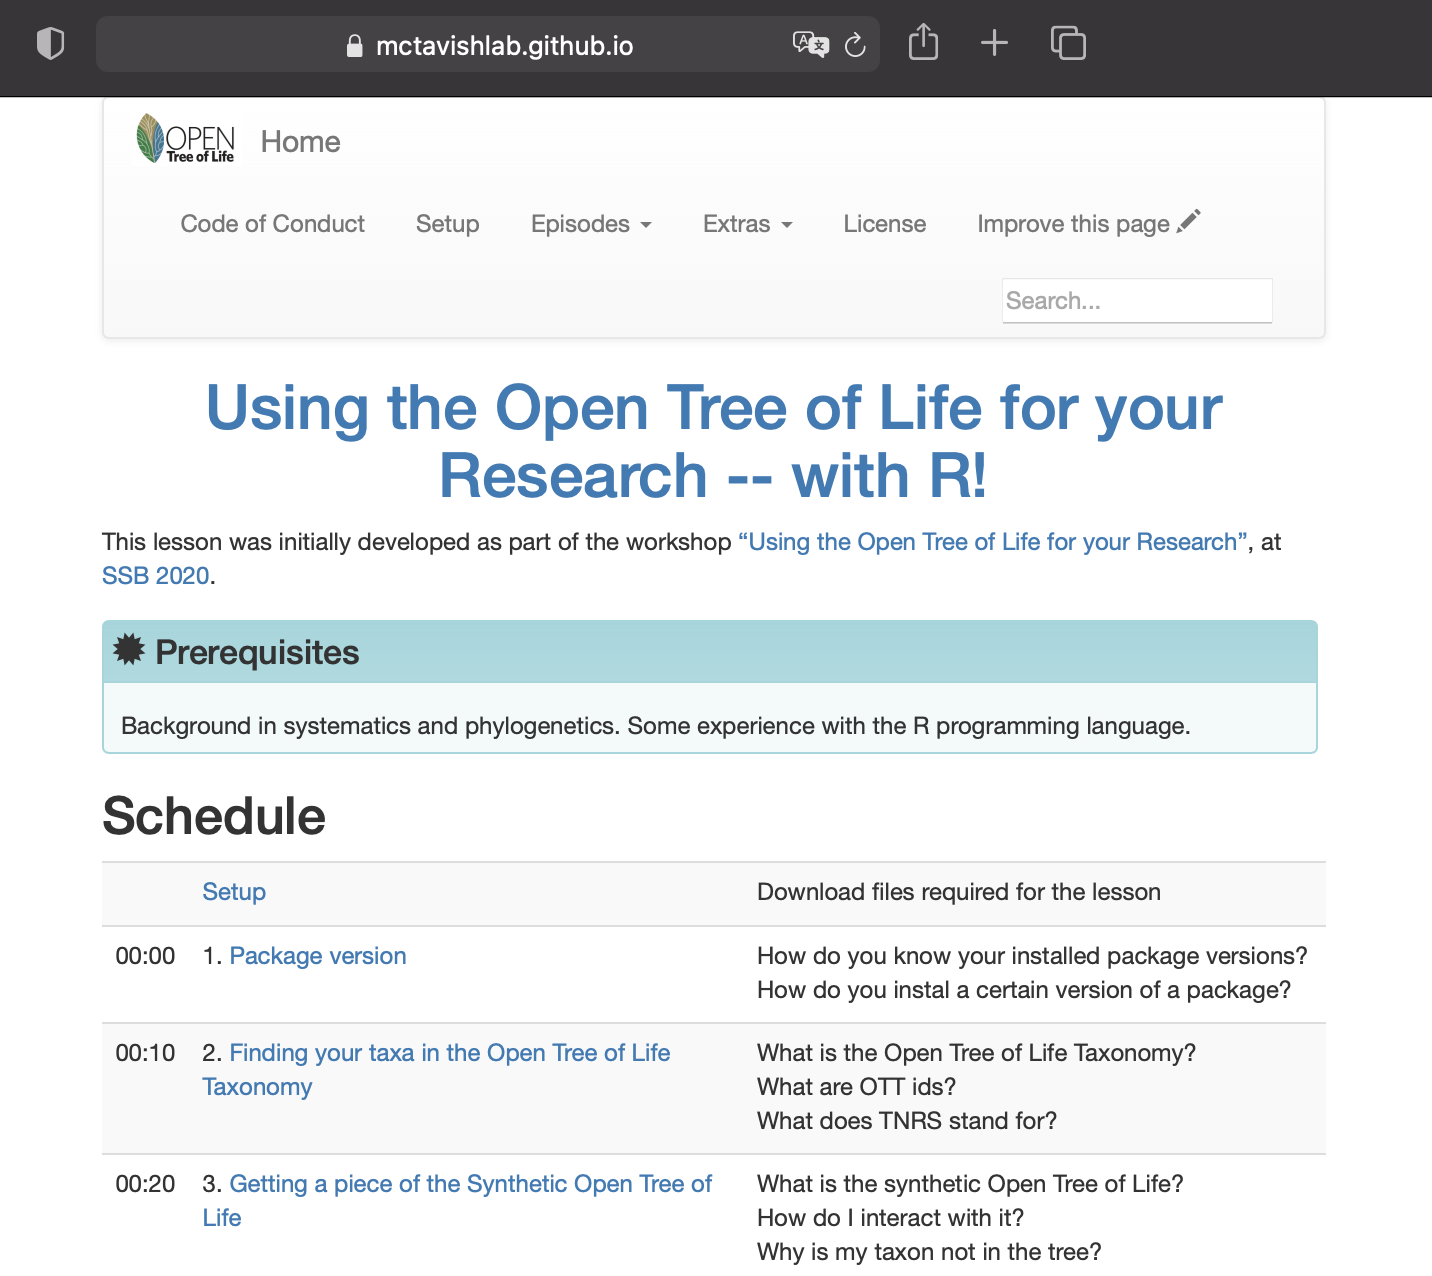
\includegraphics[width=3in]{fig_schedule.png}
\end{center}
\caption{Snapshot of the home to our tutorial website, showing part of the schedule.
 Our tutorial website was constructed using the software workshop template from the Carpentries \citep{swc-workshop-template}. \label{fig:schedule}}
\end{figure}

We note that making approachable research workflows has all the advantages of reproducible research workflows.
It saves time during explanation and training, when analyses are run by new collaborators and students.
It can also save research time for yourself, when analyses are run again with more data, a different dataset, a different organism or biological model.
It contributes to scientific efforts that can build off of each other.

% \citep{roland2002think}
Some universities and academic groups have started to incorporate reproducibility as a subject into their curriculum
\citep{uwlibraries2022, nigms2022, psyteachr2022}.
The focus of these resources has been for students to acquire and practice skills to document their work.
The principles identified and outlined here can be used to set learning goals and outcomes for new reproducibility syllabi.
Ultimately, the long term improvement of reproducibility rates in science will depend on our ability to intentionally integrate best practices for achieving reproducibility into the educational framework of future data scientists \citep{nasem2018data}.
Inclusion of reproducibility into the data acumen of undergraduate curriculum will provide college learners and future researchers with the tools to develop the fundamental skills needed to successfully create reproducible scientific workflows and research products.


The principles to create tutorials described here facilitate adoption of software and analysis workflows among researchers at different academic levels, from undergrads to established researchers.
It will also help close the gap between students that had access to computational resources (and computational training) from an early age and students that did not.
Late access to computational resources and training can occur due to lack of economic resources, often occurring in households from underrepresented communities and minorities \citep{google2016diversity, warner2021quantifying}.
It can also be due to gender-biased parental and community pressures, in which male identifying individuals are more often encouraged to perform activities related to computers, while female identifying individuals are discouraged, starting from as early as elementray school \citep{master_gender_2021}.
These principles can be used to improve not only reproducibility practices, but also software adoption in the natural sciences.


\bigskip
\begin{center}
{\large\bf SUPPLEMENTARY MATERIAL}
\end{center}

\begin{description}

\item[Title:] Website and GitHub repository containing the complete teaching materials developed and demonstrated here.

\item[GitHub repository link:] \url{https://github.com/McTavishLab/R_OpenTree_tutorials}

\item[Website link:] \url{https://mctavishlab.github.io/R_OpenTree_tutorials}

\end{description}

\bibliography{Manuscript-bibliography}

\end{document}
